\chapter{Collider Phenomenology}
In this chapter, we will discuss how to connect theory and experiment. We will begin by connecting scattering amplitudes and physically observed cross sections, after which we will briefly discuss detector components of the LHC, and then move on to the question of how we establish statistical significance given experimental data from detectors.
% Scattering amplitudes and cross sections\\
\section{Detector design for hadron colliders}

\begin{figure}[h]
  \begin{sidecaption}
    { Cutaway view of the ATLAS detector, showing the various components. Taken from \citep{Atlas2008}.}
    \centering
  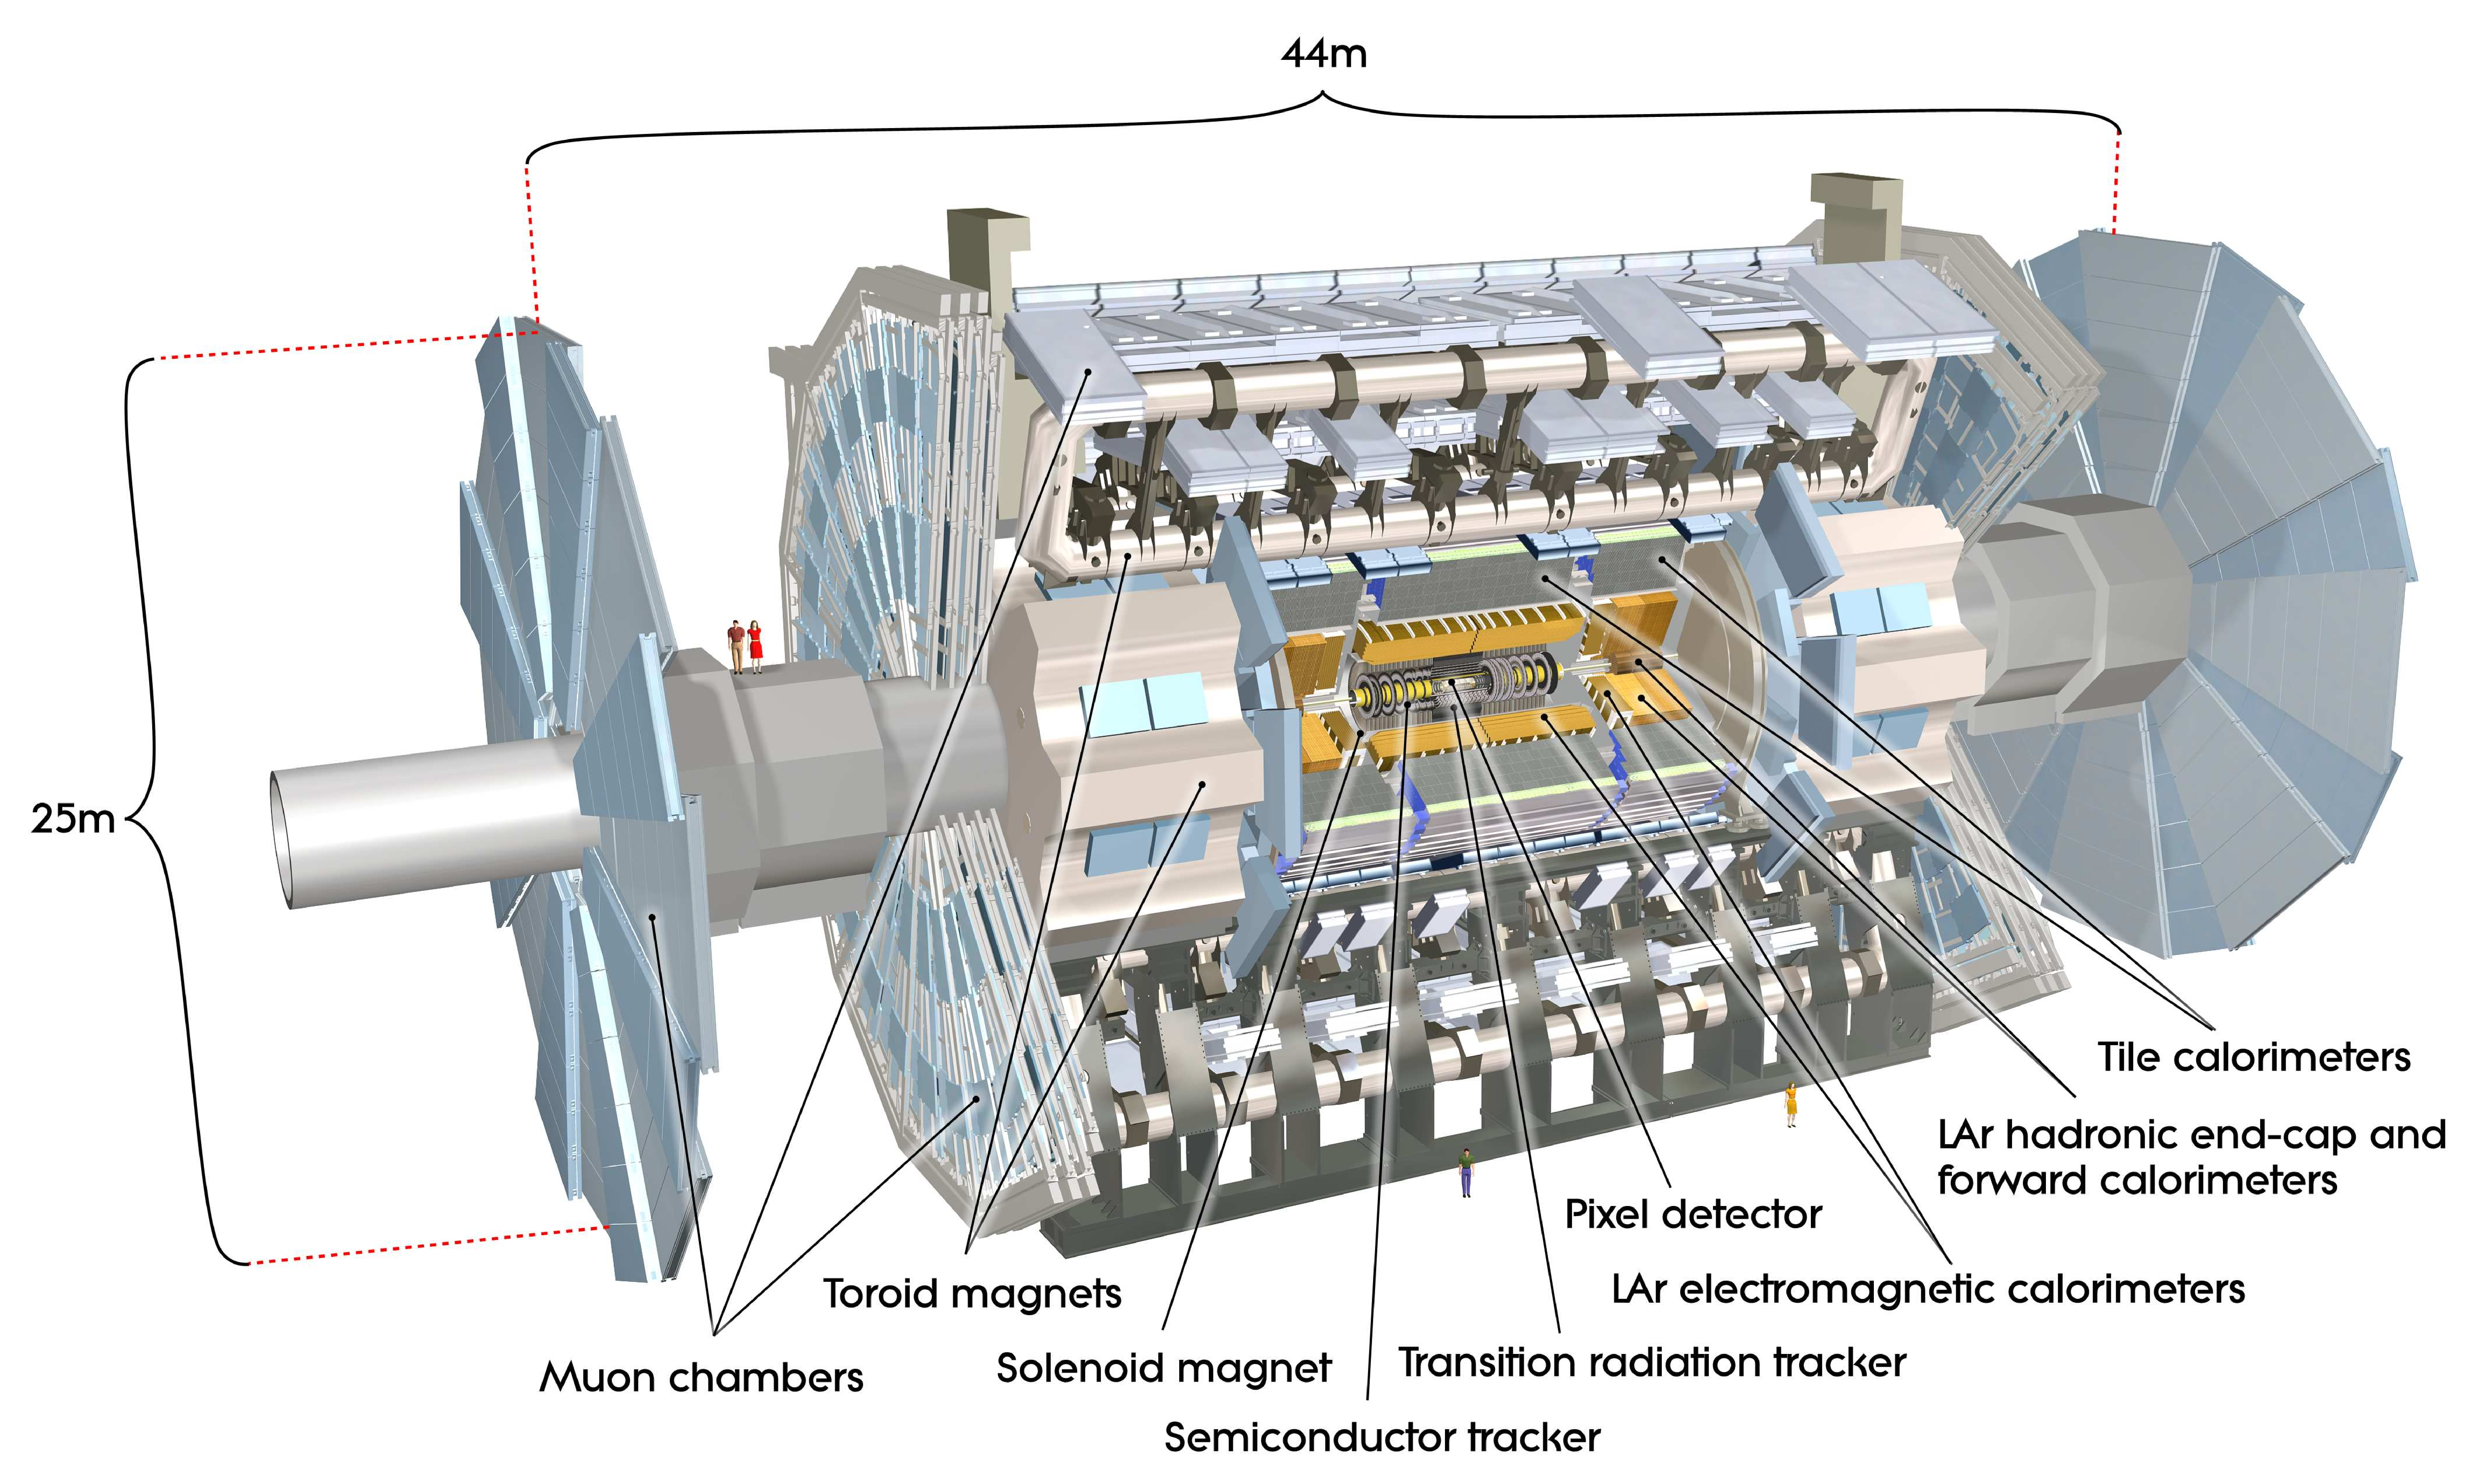
\includegraphics[trim = {2cm 5cm 2cm 2cm}, clip, width=1\textwidth]{images/atlas}
  \end{sidecaption}
\end{figure}

\section{Future circular colliders}

\begin{figure}[h]
  \begin{sidecaption}
    {Schematic diagram of the FCC ring. Tunneling under Lake Geneva will be a major challenge for the construction of the ring.}
    \centering
  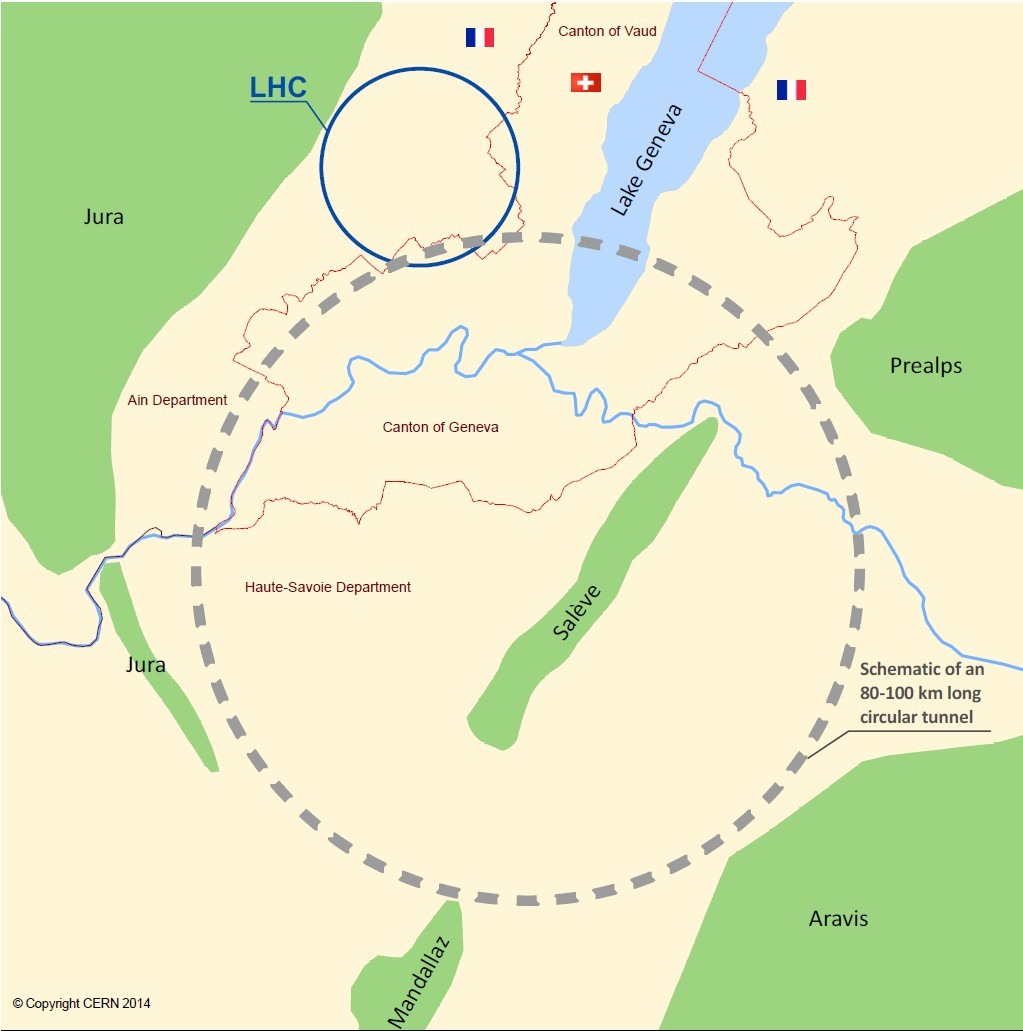
\includegraphics[width=0.9\textwidth]{images/FCC_ring_schematic}
  \end{sidecaption}
\end{figure}
\section{Anatomy of a collider analysis}
\subsection{Monte Carlo simulations}
\subsection{Showering and hadronization}
\subsection{Detector simulation and reconstruction}
\section{Statistical significance in particle physics}
